\begin{table}[h]
    \caption{Resultados da calibração dos sensores OX-B431}
    \centering
    \begin{tabularx}{0.95\textwidth}[h!]{
        >{\raggedright\hsize=.4\hsize\arraybackslash}X
        >{\raggedright\hsize=.6\hsize\arraybackslash}X 
        >{\raggedright\hsize=.6\hsize\arraybackslash}X
        >{\raggedright\hsize=.7\hsize\arraybackslash}X 
        >{\raggedright\hsize=.6\hsize\arraybackslash}X 
        >{\raggedright\hsize=.3\hsize\arraybackslash}X }
       \hline
       Var. & Modelo & R2 & RMSE & MAE & $\rho$\\ [0.5ex]
        \hline
        \acrshort{o3} (1) & \textbf{MLP}: & -0.62 ± 0.46 & -18.52 ± 2.88 & -14.33 ± 2.13 & 0.15 \\ [0.5ex]
           & \textbf{MLR} & -0.41 ± 0.29 & -17.64 ± 3.78 & -13.81 ± 2.76 & 0.14 \\ [0.5ex]
           & \textbf{KNN:} & -0.48 ± 0.32 & -18.36 ± 5.32 & -13.65 ± 4.35 & 0.13 \\ [0.5ex]
           & \textbf{RF:} & -0.61 ± 0.63 & -18.20 ± 3.30 & -14.53 ± 2.29 & 0.12 \\ [0.5ex]
        \hline
        \acrshort{o3} (1), T & \textbf{MLP:} & 0.40 ± 0.16 & -11.29 ± 1.55 & -8.71 ± 1.30 & 0.67 \\ [0.5ex]
            & \textbf{MLR:} & 0.29 ± 0.21 & -12.17 ± 1.28 & -9.50 ± 1.17 & 0.64 \\ [0.5ex]
            & \textbf{KNN:} & 0.34 ± 0.21 & -11.68 ± 1.22 & -8.92 ± 1.12 & 0.66 \\ [0.5ex]
            & \textbf{RF:} & 0.33 ± 0.19 & -11.87 ± 1.34 & -9.10 ± 1.20 & 0.63 \\ [0.5ex]
        \hline
        \acrshort{o3} (2) & \textbf{MLP}: & 0.16 ± 0.13 & -13.72 ± 2.11 & -10.87 ± 1.66 & 0.54 \\ [0.5ex]
           & \textbf{MLR} & 0.09 ± 0.14 & -14.34 ± 2.50 & -11.35 ± 2.13 & 0.56 \\ [0.5ex]
           & \textbf{KNN:} & 0.03 ± 0.35 & -14.27 +/- 1.49 & -11.27 ± 1.39 & 0.54 \\ [0.5ex]
           & \textbf{RF:} & -0.03 ± 0.37 & -14.76 ± 1.47 & -11.55 ± 1.34 & 0.52 \\ [0.5ex]
        \hline
        \acrshort{o3} (2), T & \textbf{MLP:} & 0.23 ± 0.17 & -13.16 ± 2.94 & -10.14 ± 2.62 & 0.67 \\ [0.5ex]
            & \textbf{MLR:} & 0.38 ± 0.22 & -11.44 ± 0.72 & -8.86 ± 0.86 & 0.69 \\ [0.5ex]
            & \textbf{KNN:} & 0.19 ± 0.34 & -12.91 ± 0.81 & -9.89 ± 0.92 & 0.70 \\ [0.5ex]
            & \textbf{RF:} & 0.28 ± 0.22 & -12.44 ± 1.11 & -9.54 ± 1.08 & 0.67 \\ [0.5ex]
        \hline
        \acrshort{o3} (1), \acrshort{o3} (2) & \textbf{MLP}: & 0.24 ± 0.15 & -13.01 ± 1.82 & -10.02 ± 1.55 & 0.60 \\ [0.5ex]
           & \textbf{MLR} & 0.14 ± 0.16 & -13.85 ± 2.26 & -10.81 ± 2.02 & 0.58 \\ [0.5ex]
           & \textbf{KNN:} & 0.12 ± 0.24 & -13.90 ± 1.86 & -10.86 ± 1.72 & 0.58 \\ [0.5ex]
           & \textbf{RF:} & 0.13 ± 0.24 & -13.70 ± 1.54 & -10.64 ± 1.43 & 0.57 \\ [0.5ex]
        \hline
        \acrshort{o3} (1), \acrshort{o3} (2), T & \textbf{MLP:} & 0.29 ± 0.21 & -12.37 ± 1.59 & -8.89 ± 0.82 & 0.71 \\ [0.5ex]
            & \textbf{MLR:} & 0.39 ± 0.21 & -11.37 ± 0.82 & -8.82 ± 0.88 & 0.69 \\ [0.5ex]
            & \textbf{KNN:} & 0.19 ± 0.34 & -12.97 ± 1.18 & -9.92 ± 1.37 & 0.72 \\ [0.5ex]
            & \textbf{RF:} & 0.30 ± 0.19 & -12.34 ± 1.61 & -9.57 ± 1.58 & 0.68 \\ [0.5ex]
        \hline
    \end{tabularx}
    \label{tab:data-o3-b4-calib-results}
\end{table}

% ----------------------------------------------------------
\section{Correção das leituras dos sensores OX-B431 com as medições de referência}
% ----------------------------------------------------------

A partir dos dados de referência e das leituras de concentração e temperatura adquiridas pelo monitor em questão, foi realizada uma busca em grid para encontrar as melhores combinações de parâmetros e variáveis de entrada a modelos de regressão. As variáveis que foram testadas como entrada foram as leituras de concentração de \acrshort{o3} dos dois sensores OX-B431 e a temperatura no interior da câmara de medição. Na Tabela \ref{tab:data-o3-b4-calib-results} resumem-se os melhores modelos encontrados pela busca em \textit{grid} para calibrar as leituras dos sensores OX-B431. São mostradas as diferentes combinações de variáveis de entrada testadas em cada iteração da busca pelos melhores modelos de regressão. Os mesmos resultados são ilustrados graficamente na Figura \ref{fig:data-o3-b4-models-performance} que apresenta o desempenho dos modelos e as variáveis de entrada considerando os valores de R2, RMSE e MAE.

\begin{figure}[h!]
    \centering
    \caption{Resultados dos modelos de regressão aplicados às leituras dos sensores OX-B431}
    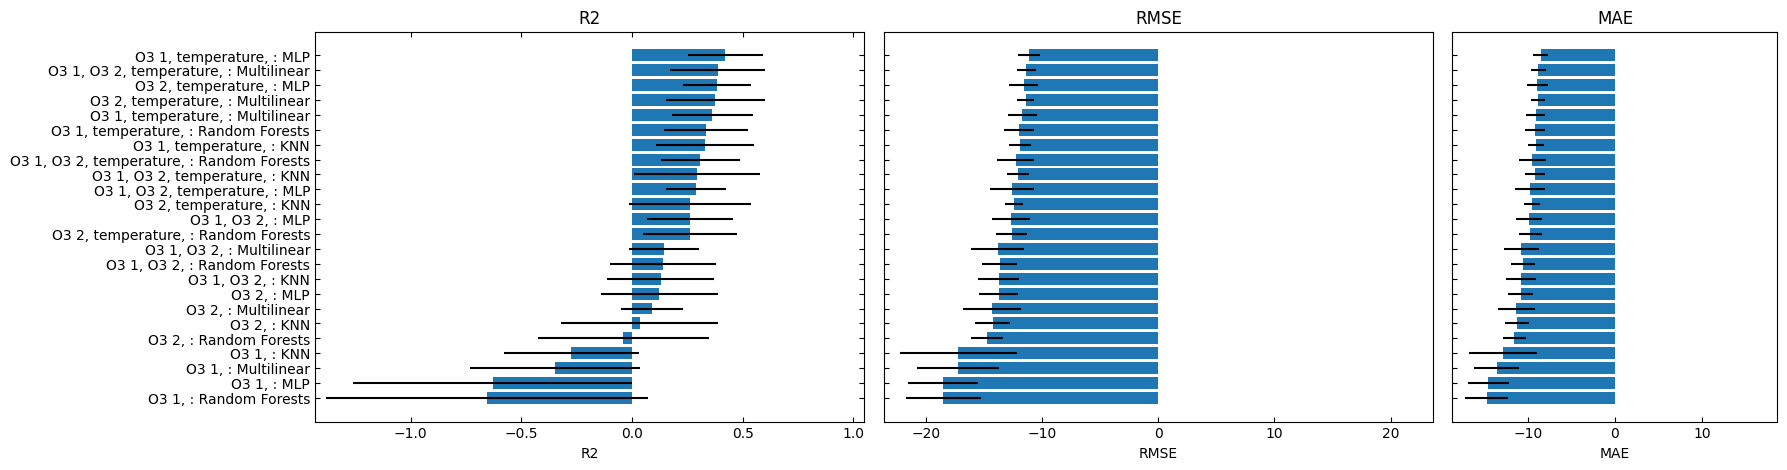
\includegraphics[width=\textwidth]{chapters/4-CALIBRAÇÃO MÚLTIPLOS SENSORES/Figuras/o3-b4-models-performance.png}
    \label{fig:data-o3-b4-models-performance}
\end{figure}

\begin{figure}[h!]
    \centering
    \caption{Gráfico de dispersão das leituras dos sensores de \acrshort{o3} OX-B431 e a estação de referência após aplicar modelos de regressão considerando a temperatura}
    \begin{subfigure}{0.49\textwidth}
        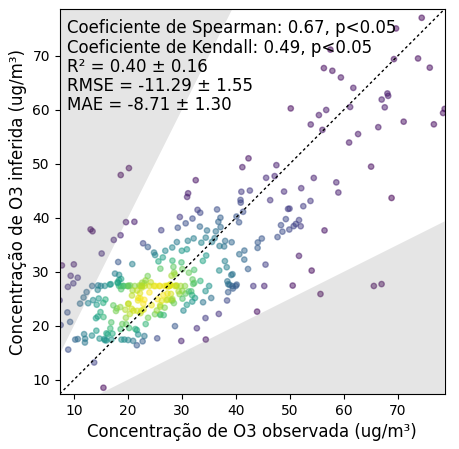
\includegraphics[width=\textwidth]{chapters/4-CALIBRAÇÃO MÚLTIPLOS SENSORES/Figuras/o3-b4-1-T-MLP-Regression.png}
        \caption{Utilizando uma rede neural Perceptron Multicamadas obtiverem-se os melhores resultados de R2, RMSE e MAE considerando as leituras do sensor 1 e a temperatura}
        \label{fig:data-o3-1-T-reference-corr-MLP}
    \end{subfigure}
    \hfill
    \begin{subfigure}{0.49\textwidth}
        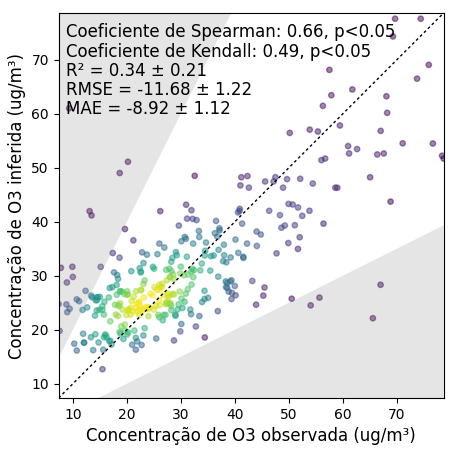
\includegraphics[width=\textwidth]{chapters/4-CALIBRAÇÃO MÚLTIPLOS SENSORES/Figuras/o3-b4-1-T-KNN-Regression.png}
        \caption{Utilizando uma regressão pelos k vizinhos mais próximos considerando as leituras do sensor 1 e a temperatura obtiveram-se resultados semelhantes}
        \label{fig:data-o3-1-2-T-reference-corr-MLR}
    \end{subfigure}
\end{figure}

De modo geral observa-se que os modelos que consideraram a temperatura como variável de entrada produziram os melhores resultados de R2, erro e correlação. A dupla de variáveis sensor OX-B431 (1) e temperatura ocupou os primeiros lugares com diferentes modelos de regressão. Ao remover a temperatura, os modelos que melhor desempenharam consideraram os dois sensores de \acrshort{o3}; os sensores individualmente não produziram bons resultados. As Figuras \ref{fig:data-o3-1-T-reference-corr-MLP} e \ref{fig:data-o3-1-2-T-reference-corr-MLR} apresentam gráficos de dispersão com as leituras de referência e as inferidas pelos dois melhores modelos em termos de R2, RMSE e MAE.

\begin{figure}[h!]
    \centering
    \caption{Desempenho dos modelos de regressão aplicados para inferir as leituras de concentração de \acrshort{o3} medidas pela estação de referência}
    \begin{subfigure}{0.9\textwidth}
        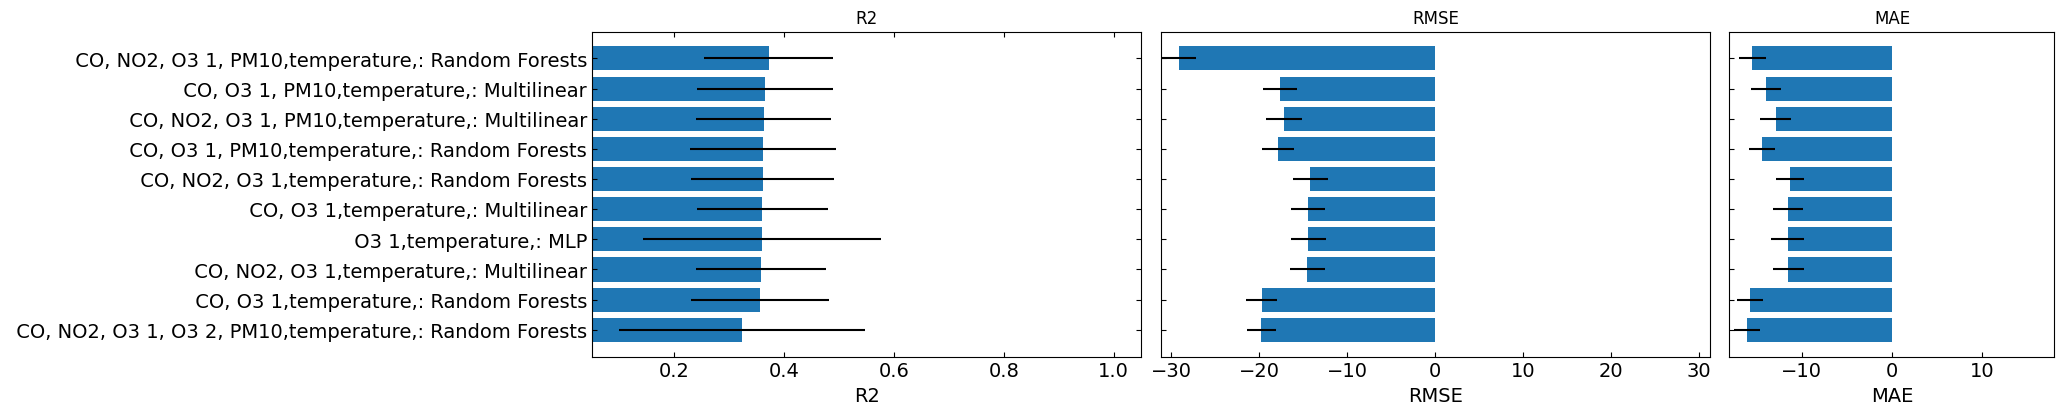
\includegraphics[width=\textwidth]{chapters/4-CALIBRAÇÃO MÚLTIPLOS SENSORES/Figuras/o3-all-models-performance.png}
        \caption{Valores de R2, RMSE e MAE obtidos pelos 10 modelos com maiores valores de R2}
        \label{fig:data-o3-all-models-performance}
    \end{subfigure}
    \begin{subfigure}{0.9\textwidth}
        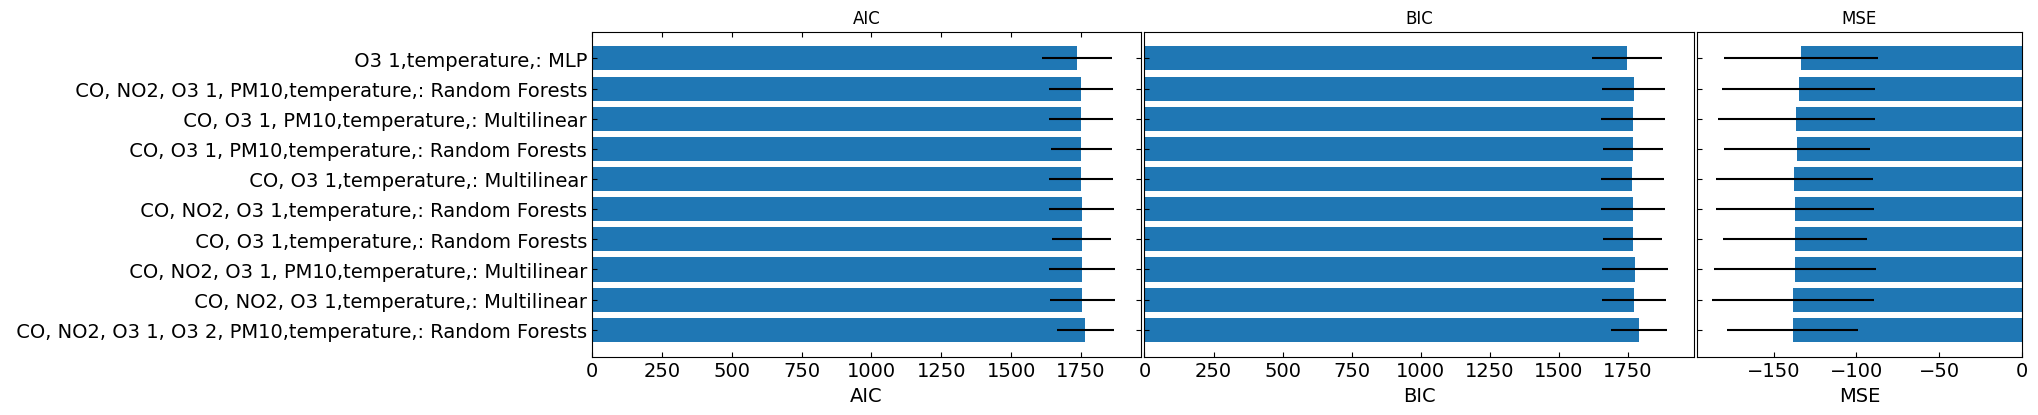
\includegraphics[width=\textwidth]{chapters/4-CALIBRAÇÃO MÚLTIPLOS SENSORES/Figuras/o3-all-models-complexity.png}
        \caption{Modelos com menores valores de \acrshort{aic} e \acrshort{bic}}
        \label{fig:data-o3-all-models-comlexity}
    \end{subfigure}
    \label{fig:data-o3-all-models-performance-comlexity}
\end{figure}

\begin{figure}[h]
    \centering
    \caption{Gráfico de dispersão das leituras do múltiplos sensores e a estação de referência para medição de \acrshort{o3}}
    \begin{subfigure}{0.49\textwidth}
        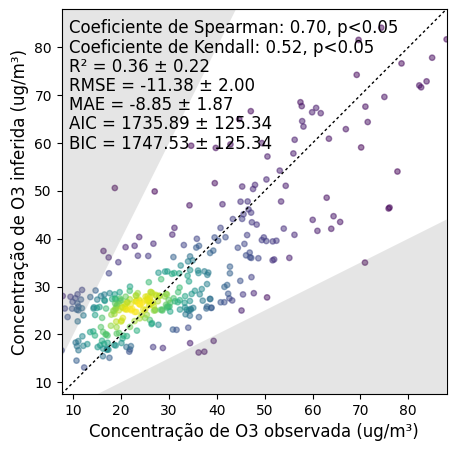
\includegraphics[width=\textwidth]{chapters/4-CALIBRAÇÃO MÚLTIPLOS SENSORES/Figuras/O3-o31-T-MLP-Regression.png}
        \caption{Utilizando uma rede neural perceptron multicamadas com variáveis independentes: leituras de sensor OX-B431 (1) e temperatura}
        \label{fig:data-o31-T-reference-O3-corr-MLP}
    \end{subfigure}
    \hfill
    \begin{subfigure}{0.49\textwidth}
        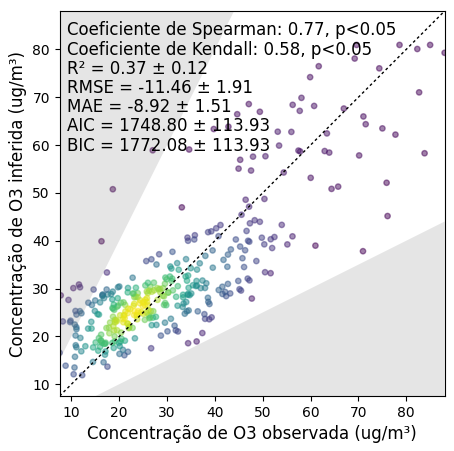
\includegraphics[width=\textwidth]{chapters/4-CALIBRAÇÃO MÚLTIPLOS SENSORES/Figuras/O3-co-no2-o31-pm10-T-RF-Regression.png}
        \caption{Utilizando modelo de regressão de Florestas Aleatórias com variáveis independentes: leituras de sensores CO-B4, NO2-B43F, OX-B431 (1), sensor de \acrshort{mp10} OPC-N3 e temperatura}
        \label{fig:data-co-no2-o31-pm10-T-reference-O3-corr-RF}
    \end{subfigure}
\end{figure}

% ----------------------------------------------------------
\section{Cálculo da concentração de Ozônio a partir das leituras do arranjo de sensores de gases}
% ----------------------------------------------------------

As Figuras \ref{fig:data-o3-all-models-performance} e \ref{fig:data-o3-all-models-comlexity} apresenta os valores de R2, RMSE, MAE, AIC e BIC dos 10 melhores modelos de calibração calculados para as leituras de \acrshort{o3}. Observa-se que os valores de R2 desses 10 modelos oscilaram entre 0.1 e 0.6, e que todos incluíram a temperatura. O Perceptron Multicamadas que considerou apenas as leituras do sensor OX-B431 (1) e a temperatura gerou o maior valor de R2 = 0.6, mas também gerou um dos menores de aproximadamente 0.1. Este modelo também apresentou a menor complexidade em termos de coeficientes AIC e BIC. O modelo que teve o maior valor de R2 médio também apresentou o maior erro médio quadrático, e os que se encontraram nas posições 5 - 8 geraram os menores valores de RMSE. A Figura \ref{fig:data-o31-T-reference-O3-corr-MLP} mostra os resultados de aplicar uma rede neural Perceptron Multicamadas com variáveis de entrada OX-B431 (1) e temperatura, que gerou o maior R2, um dos menores RMSE e menor complexidade. A Figura \ref{fig:data-co-no2-o31-pm10-T-reference-O3-corr-RF}, por usa parte, mostra os resultados obtidos com Florestas Aleatórias e variáveis de entrada CO-B4, NO2-B43F, OX-B431 (1), \acrshort{mp10} do OPC-N3 e temperatura, que foi a combinação com maior R2 médio e a segunda com menor complexidade segundo os valores de AIC e BIC.